%&pdflatex
\documentclass[12pt]{article}
\usepackage[margin=1.0in]{geometry}

\usepackage{g-util}
\usepackage{amsfonts, amsmath, amssymb}
\usepackage{graphicx, float}
\graphicspath{ {../data/} }
%\usepackage[xetex]{xcolor}

\setcounter{MaxMatrixCols}{12}
\newcommand{\Gpmatrix}[1]{\ensuremath{\begin{pmatrix} #1 \end{pmatrix}}}
\newcommand{\Gbmatrix}[1]{\ensuremath{\begin{bmatrix} #1 \end{bmatrix}}}
\newcommand{\sub}[3]{\ensuremath{#1_{#2,#3}}}
\newcommand{\supra}[2]{\ensuremath{#1^#2}}

\title{Métodos Numéricos}
\author{F. Galileo Cappella Lewi}
\date{1c2022}

\renewcommand{\figurename}{Fig.}
\renewcommand{\listfigurename}{Figuras}
\renewcommand{\contentsname}{Secciones}

\begin{document}

\maketitle

\section{Introducción}

%TODO: Contar el problema que nos presentaron
En general vamos a estar trabajando con \(m+1\) radios, y \(n\) ángulos.

\section{Formulación del Sistema}
 
\paragraph{} Partimos de la ecuación de Laplace \\
\[
  0 = \frac{\partial^2T(r,\ \theta)}{\partial r^2} + \frac{1}{r} \frac{\partial^2T(r,\ \theta)}{\partial r} + \frac{1}{r^2} \frac{\partial^2T(r,\ \theta)}{\partial\theta^2}
\]
Y la discretizamos \\ %TODO: Pasos y justificación en el medio?
\[
0 = \frac{\sub{t}{j-1}{k} - 2\sub{t}{j}{k} + \sub{t}{j+1}{k}}{(\Delta r)^2} + \frac{\sub{t}{j}{k} - \sub{t}{j-1}{k}}{r \Delta r} + \frac{\sub{t}{j}{k-1} - 2\sub{t}{j}{k} + \sub{t}{j}{k+1}}{r^2 (\Delta \Theta)^2}
\]
Podemos reescribir la ecuación como una combinación lineal de cinco temperaturas \\
\begin{align} %TODO: Más chiquita
0 = \sub{t}{j-1}{k} (\frac{1}{(\Delta r)^{2}} + \frac{-1}{r \Delta r}) + \sub{t}{j}{k} (\frac{-2}{(\Delta r)^2} + \frac{1}{r \Delta r} + \frac{-2}{(r \Delta \Theta)^{2}}) + \sub{t}{j+1}{k} \frac{1}{(\Delta r)^{2}} + \sub{t}{j}{k-1} \frac{1}{(r \Delta \Theta)^{2}} + \sub{t}{j}{k+1} \frac{1}{(r\Delta \Theta)^{2}}
\end{align}
Para simplificar la notación vamos a nombrar cada coeficiente \\ %TODO: Renombrar coeficientes para que tengan más sentido
\(
\tab \alpha_r = \frac{1}{(\Delta r)^{2}} + \frac{-1}{r \Delta r} \\
\tab \beta_r = \frac{-2}{(\Delta r)^2} + \frac{1}{r \Delta r} + \frac{-2}{(r \Delta \Theta)^{2}} \\
\tab \gamma_r = \frac{1}{(\Delta r)^{2}} \\ 
\tab \chi_r = \frac{1}{(r \Delta \Theta)^{2}}
\) \\\\
Resaltamos cuatro formas diferentes de escribir la ecuación \\
\begin{align}
  \alpha \sub{t}{j-1}{k} + \beta \sub{t}{j}{k} + \gamma \sub{t}{j+1}{k} + \chi \sub{t}{j}{k-1} + \chi \sub{t}{j}{k+1} = 0 \\
  \beta \sub{t}{j}{k} + \gamma \sub{t}{j+1}{k} + \chi \sub{t}{j}{k-1} + \chi \sub{t}{j}{k+1} = -\alpha \sub{t}{j-1}{k} \\
  \alpha \sub{t}{j-1}{k} + \beta \sub{t}{j}{k} + \chi \sub{t}{j}{k-1} + \chi \sub{t}{j}{k+1} = -\gamma \sub{t}{j+1}{k} \\
  \beta \sub{t}{j}{k} + \chi \sub{t}{j}{k-1} + \chi \sub{t}{j}{k+1} = -\alpha \sub{t}{j-1}{k} - \gamma \sub{t}{j+1}{k}
\end{align}
\\
\paragraph{} Por lo que podemos armar un sistema de ecuaciones de la forma \(Ax = b\) donde cada fila del sistema se corresponde a una instancia de la ecuación de Laplace discretizada. \\
Pero qué forma tiene cada instancia depende de si la temperatura del radio anterior o la del siguiente también son incógnitas (por lo que tienen su coeficiente en la matriz), o si son datos medidos (por lo que cambian al resultado): \\
\tab El primer y último radios (\(\sub{t}{1}{k}\) y \(\sub{t}{m+1}{k}\)) son datos medidos, por lo que no hace falta estimarlos con una ecuación. \\
\tab Como las temperaturas del radio anterior las conocemos (porque son las temperaturas internas medidas), las primeras \(n\) filas (que se corresponden con el radio \(\sub{t}{2}{k}\)) van a tener la forma de la ecuación (3). \\ %TODO: Hyperlink
\tab Luego, las siguientes \((m-2)n\) filas (que son todos los otros radios excepto el \(\sub{t}{m}{k}\)) tienen tanto al radio anteriro como el siguiente incógnitas, por lo que tienen la forma de la ecuación (2). \\ %TODO: Hyperlink
\tab Y las últimas \(n\) filas (radio \(\sub{t}{m}{k}\)) tienen la forma de la ecuación (4). \\ %TODO: Hyperlink
Entonces nos queda una matriz \(A \in \mathbb{R}^{((m-1)n \times (m-1)n)}\) armada de la forma explicada recién, el vector de incógntias \(x \in \mathbb{R}^{(m-1)n}\) con los radios "estirados" uno arriba del otro, y el vector de resultados \(b \in \mathbb{R}^{(m-1)n}\) que tiene las temperaturas medidas en las primeras y últimas \(n\) filas, y el resto 0's.

\paragraph{} El caso de un sistema con 3 radios es especial, ya que para el radio \(\sub{t}{2}{k}\) (que es el vector de incógnitas completo) conocemos tanto las temperaturas del radio anterior como del siguiente. Sólo en este caso tenemos la ecuación (5).

\subsection{Justificación no-pivoteo} 
\label{sec:justificacion}

%TODO

\subsection{Ejemplos}

\paragraph{3 radios y 4 ángulos:} \ \\

\(
\Gpmatrix{
  \beta & \chi & 0 & \chi \\
  \chi & \beta & \chi & 0 \\
  0 & \chi & \beta & \chi \\
  \chi & 0 & \chi & \beta \\
} \cdot \Gpmatrix{
  \sub{t}{2}{1} \\
  \sub{t}{2}{2} \\
  \sub{t}{2}{3} \\
  \sub{t}{2}{4} \\
} = \Gpmatrix{
  -\alpha\sub{t}{1}{1} - \gamma\sub{t}{3}{1} \\
  -\alpha\sub{t}{1}{2} - \gamma\sub{t}{3}{2} \\
  -\alpha\sub{t}{1}{3} - \gamma\sub{t}{3}{3} \\
  -\alpha\sub{t}{1}{4} - \gamma\sub{t}{3}{4} \\
}
\)

%\paragraph{4 radios y 4 ángulos:} \ \\

%\(
%\Gpmatrix{
  %\beta & \chi & 0 & \chi & -\gamma & 0 & 0 & 0 \\
  %\chi & \beta & \chi & 0 & 0 & -\gamma & 0 & 0 \\
  %0 & \chi & \beta & \chi & 0 & 0 & -\gamma & 0 \\
  %\chi & 0 & \chi & \beta & 0 & 0 & 0 & -\gamma \\
  %-\alpha & 0 & 0 & 0 & \beta & \chi & 0 & \chi \\
  %0 & -\alpha & 0 & 0 & \chi & \beta & \chi & 0 \\
  %0 & 0 & -\alpha & 0 & 0 & \chi & \beta & \chi \\
  %0 & 0 & 0 & -\alpha & \chi & 0 & \chi & \beta \\
%} \cdot \Gpmatrix{
  %\sub{t}{2}{1} \\
  %\sub{t}{2}{2} \\
  %\sub{t}{2}{3} \\
  %\sub{t}{2}{4} \\
  %\sub{t}{3}{1} \\
  %\sub{t}{3}{2} \\
  %\sub{t}{3}{3} \\
  %\sub{t}{3}{4} \\
%} = \Gpmatrix{
  %-\alpha\sub{t}{1}{1} \\
  %-\alpha\sub{t}{1}{2} \\
  %-\alpha\sub{t}{1}{3} \\
  %-\alpha\sub{t}{1}{4} \\
  %-\gamma\sub{t}{4}{1} \\
  %-\gamma\sub{t}{4}{2} \\
  %-\gamma\sub{t}{4}{3} \\
  %-\gamma\sub{t}{4}{4} \\
%}
%\)

\paragraph{5 radios y 4 ángulos:} \ \\

\(
\Gpmatrix{
  \beta & \chi & 0 & \chi & -\gamma & 0 & 0 & 0 & 0 & 0 & 0 & 0 \\
  \chi & \beta & \chi & 0 & 0 & -\gamma & 0 & 0 & 0 & 0 & 0 & 0 \\
  0 & \chi & \beta & \chi & 0 & 0 & -\gamma & 0 & 0 & 0 & 0 & 0 \\
  \chi & 0 & \chi & \beta & 0 & 0 & 0 & -\gamma & 0 & 0 & 0 & 0 \\
  -\alpha & 0 & 0 & 0 & \beta & \chi & 0 & \chi & -\gamma & 0 & 0 & 0 \\
  0 & -\alpha & 0 & 0 & \chi & \beta & \chi & 0 & 0 & -\gamma & 0 & 0 \\
  0 & 0 & -\alpha & 0 & 0 & \chi & \beta & \chi & 0 & 0 & -\gamma & 0 \\
  0 & 0 & 0 & -\alpha & \chi & 0 & \chi & \beta & 0 & 0 & 0 & -\gamma \\
  0 & 0 & 0 & 0 & -\alpha & 0 & 0 & 0 & \beta & \chi & 0 & \chi \\
  0 & 0 & 0 & 0 & 0 & -\alpha & 0 & 0 & \chi & \beta & \chi & 0 \\
  0 & 0 & 0 & 0 & 0 & 0 & -\alpha & 0 & 0 & \chi & \beta & \chi \\
  0 & 0 & 0 & 0 & 0 & 0 & 0 & -\alpha & \chi & 0 & \chi & \beta \\
} \cdot \Gpmatrix{
  \sub{t}{2}{1} \\
  \sub{t}{2}{2} \\
  \sub{t}{2}{3} \\
  \sub{t}{2}{4} \\
  \sub{t}{3}{1} \\
  \sub{t}{3}{2} \\
  \sub{t}{3}{3} \\
  \sub{t}{3}{4} \\
  \sub{t}{4}{1} \\
  \sub{t}{4}{2} \\
  \sub{t}{4}{3} \\
  \sub{t}{4}{4} \\
} = \Gpmatrix{
  -\alpha\sub{t}{1}{1} \\
  -\alpha\sub{t}{1}{2} \\
  -\alpha\sub{t}{1}{3} \\
  -\alpha\sub{t}{1}{4} \\
  0 \\
  0 \\
  0 \\
  0 \\
  -\gamma\sub{t}{5}{1} \\
  -\gamma\sub{t}{5}{2} \\
  -\gamma\sub{t}{5}{3} \\
  -\gamma\sub{t}{5}{4} \\
}
\)
\subsection{Implementación}

Implementamos este sistema en \texttt{C++}, y luego analizamos los resultados con \texttt{Python}.

\begin{figure}[H]
\centering
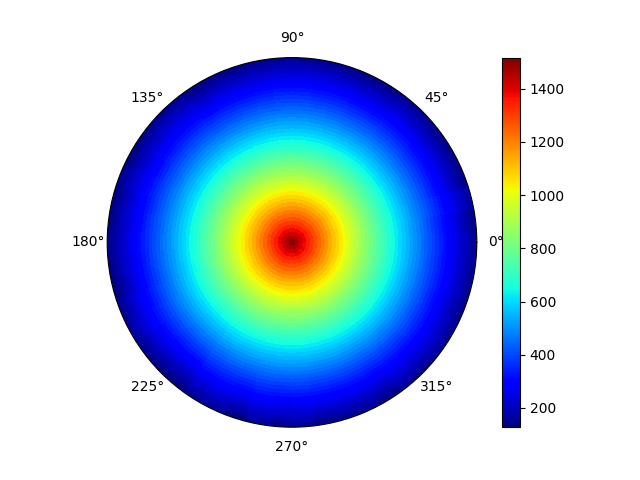
\includegraphics[width=\textwidth]{test.0}
\caption{Temperatura dentro del horno}
\label{fig:temperature}
\end{figure}

%\subsection{Matriz en "banda"}
%%TODO

\section{Gauss vs LU}

\paragraph{} Para resolver un sistema de ecuaciones cualquiera planteado como \(Ax = b\), se puede usar el método de eliminación gausseana (o "Gauss"), que tiene un tiempo de operación \(\bigO{n^3}\). Pero también se puede resolver usando la factorización \(LU\), que son dos matrices tales que \(A = LU\), y \(L\) es triangular inferior y \(U\) triangular superior. La forma de resolverlo así sería primero calcular un \(y\) tal que \(Ly = b\) y luego resolver \(Ux = y\). Esto toma \(\bigO{n^2}\) operaciones.
\paragraph{} Como vimos en la sección \ref{sec:justificacion}, la matriz de nuestro sistema tiene factorización \(M = LU\). Lo cual nos es muy útil cuando queremos resolver múltiples instancias de \(Mt_i = b_i\) ya que la factorización \(LU\) se puede calcular aplicando Gauss una sola vez, y resolver cada instancia \(LUt_i = b_i\) requiere muchas menos operaciones. \\
En la figura \ref{fig:solve.time} se puede ver que una vez que la matriz tiene 30 o más elementos, se vuelve definitivamente mejor resolver una instancia con \(LU\) que con Gauss. 

\begin{figure}[H]
\centering
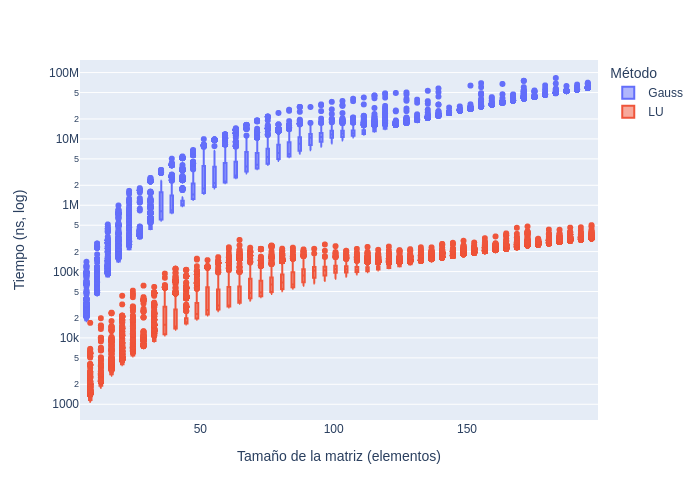
\includegraphics[width=\textwidth]{times.solve}
\caption{Tiempo para resolver una instancia del sistema (1000 reps)}
\label{fig:solve.time}
\end{figure}

\begin{figure}[H]
\centering
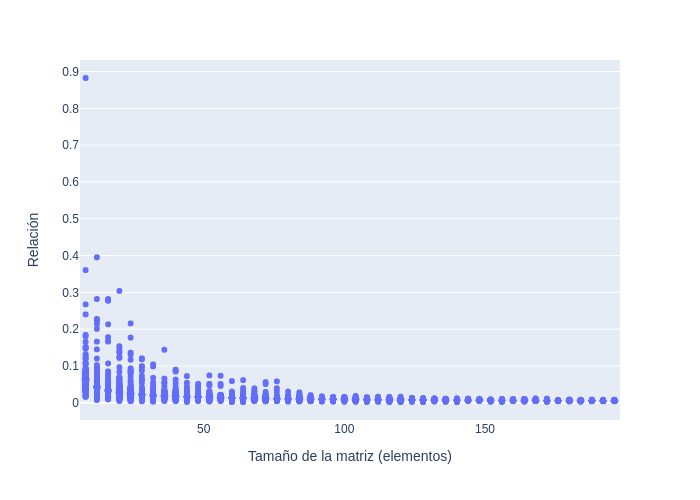
\includegraphics[width=\textwidth]{times.ratio_lu_gauss}
\caption{Relación del tiempo entre LU y Gauss (1000 reps)}
\label{fig:solve.time.ratio}
\end{figure}


\paragraph{} Pero como mencionamos, para calcular la factorización hay que aplicar Gauss una vez, por lo que en realidad nos queda el resultado de la figura \ref{fig:solve.lu.time} para resolver una instancia. \\
Por lo que es importante revisar cuándo de verdad nos empieza a convenir usar la factorización \(LU\). En la figura \ref{fig:pct_lu.time} se ve que independiente del tamaño de la matriz, el tiempo usado para resolver una instancia del sistema es una fracción mínima del tiempo usado para calcular la factorización. %TODO: Cuánto te combiene para la más chiquita

%TODO: Gráfico de sumando lu

%\begin{figure}[H]
%\centering
%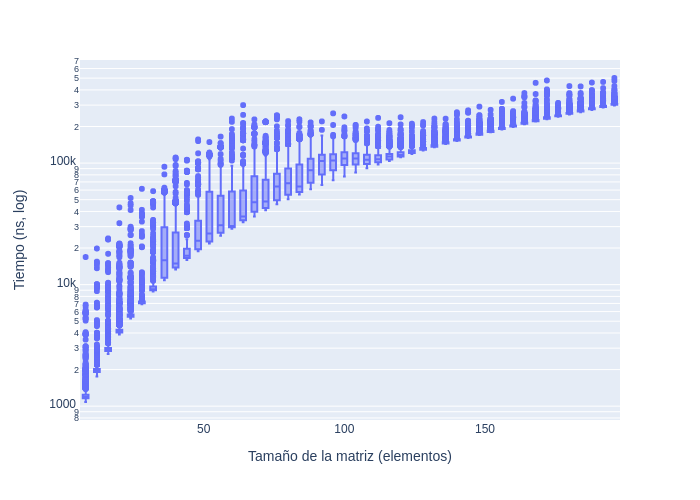
\includegraphics[width=\textwidth]{times.lu}
%\caption{Tiempo para calcular la factorización LU (1000 reps)}
%\label{fig:lu.time}
%\end{figure}

\begin{figure}[H]
\centering
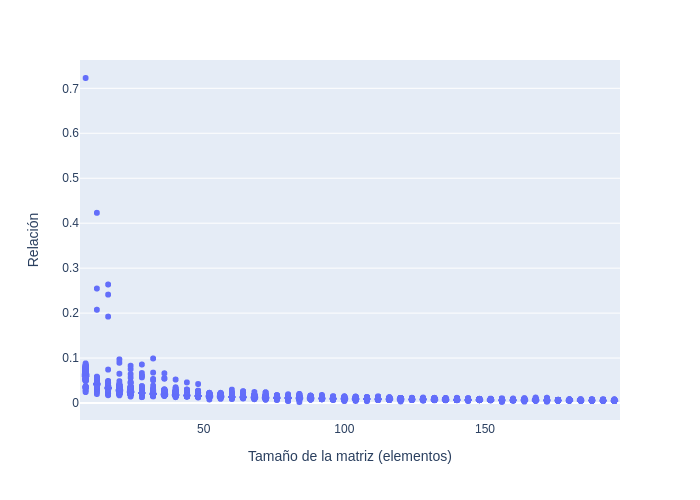
\includegraphics[width=\textwidth]{times.pct_lu}
\caption{Relación entre el tiempo para resolver el sistema y el tiempo para calcular la factorización LU (1000 reps)}
\label{fig:pct_lu.time}
\end{figure}

\section{Estimando la isoterma}

\paragraph{} Un dato importante que nos interesa es encontrar la posición de la isoterma de 500ºC. Esta es un círculo dentro de la pared del horno todo a la misma temperatura. \\
Queremos poder calcularla porque si está "muy cerca" (ver sección \ref{sec:peligrosidad.distance}) la estructura del horno estaría en riesgo. %TODO: Hyperlink

\begin{figure}[H]
\centering
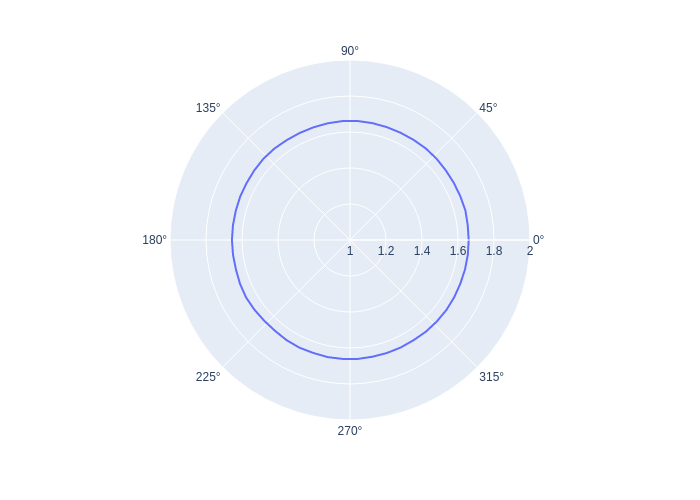
\includegraphics[width=\textwidth]{test.isotherm.0}
\caption{Posición de la isoterma}
\label{fig:isotherm.pos}
\end{figure}

\paragraph{} Para encontarla buscamos dos puntos dentro de un mísmo ángulo que "rodeen" la temperatura buscada, y luego aproximamos linealmente la posición donde se encuentra entre estos dos puntos.

%TODO: Diagrama mostrando la isoterma estimada entre dos puntos

\subsection{Midiendo la Peligrosidad}
\label{sec:peligrosidad.distance}

\paragraph{} Una vez encontrada la isoterma, es importante decidir si el horno está en un estado peligroso o seguro. Sabemos que si el exterior del horno llega a tener una temperatura de 500ºC o más, se rompe. \\
En la figura \ref{fig:peligrosidad.distance} se puede ver cómo se mueve la isoterma de 500ºC si la temperatura interna creciera uniformemente. \\

\begin{figure}[H]
\caption{Distancia de la isoterma al exterior del horno}
\centering
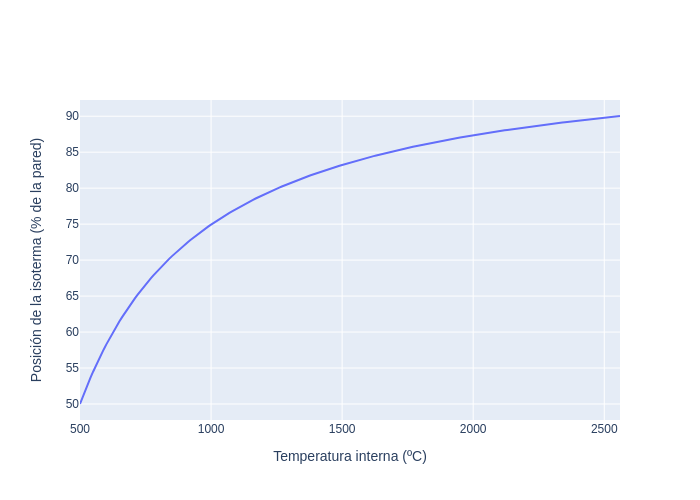
\includegraphics[width=\textwidth]{peligrosidad.distance}
\label{fig:peligrosidad.distance}
\end{figure}

\paragraph{} Para sacar conclusiones sobre qué tan peligroso es, habría que conocer más sobre los materiales que forman al horno. Pero preliminarmente se puede ver que si el "punto de ruptura" se encuentra al 75\% hay poco margen de error, ya que la isoterma se mueve rápido hacia el exterior.

\section{Apéndice}

\tableofcontents

\listoffigures

\end{document}

%TODO: Math formatting
